\section{Spanning Trees}
\subsection{Preliminaries}

A spanning tree $T$ of a graph $G$ is a subgraph of $G$ that is a tree and contains all nodes. In a spanning tree any pair of vertices $(u,v)$ is connected by a unique path. Having unique paths in computer networks makes it possible to route messages more efficiently. Obviously some spanning trees are more useful for communication than others, cf figure \ref{fig:not_all_trees_equal}. Graphs/spanning trees with small diameter\footnote{The length of the longest shortest path between any two nodes in the graph} are desirable.

\begin{figure}[hbt]
\begin{center}
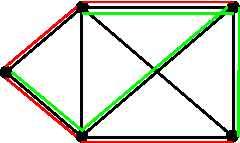
\includegraphics[scale=1.5]{./images/not_all_trees_equal}
\end{center}
\caption{The green tree is more desirable since the diameter is smaller}
\label{fig:not_all_trees_equal}
\end{figure}

Recall that in unweighted graphs the BFS tree is a tree of shortest paths from the root to all other vertices.

\begin{lem} If $T$ is a spanning tree of $G$, the diameter of $T$ is at least as large as the diameter of $G$.\end{lem}

\begin{pr} Obvious, since $T$ is obtained by removing edges from $G$, paths can only get longer.\end{pr}

The gap between the diameter of $G$ and a spanning tree $T$ can be on the order of $n$, cf. figure \ref{fig:diameter_ratio_spanning_tree}. For BFS trees its not so bad though.

\begin{figure}
\begin{center}
\includegraphics{./images/diameter_ratio_spanning_tree}
\end{center}
\caption{An example for a bad spanning tree}
\label{fig:diameter_ratio_spanning_tree}
\end{figure}

\begin{lem} The diameter of a BFS tree $T$ is at most twice the diameter of $G$\end{lem}
\begin{pr} In any tree $T$ the following holds for the distances:

\[d_T(u,v) \leq d_T(u,r) + d_T(r,v)\]

Since the BFS tree is a tree of shortest paths from the root, we have $d_T(u,r), d_T(r,v) = d_G(u,r), d_G(r,v)$. Since both distances are smaller than the diameter, the bound follows\end{pr} 

\subsection{Broadcasting and Spanning Trees}

Suppose we have a graph $G$ with a node $r\in V$ that wants to broadcast something to all other nodes. Let $D$ be the diameter of $G$ and $R$ be the radius\footnote{The maximal distance of a node to $r$} of $r$. Note $R\leq D\leq 2R$.

\begin{figure}
\begin{lstlisting}
wait for message
forward the message to all other neighbours 
//no loop!
\end{lstlisting}
\caption{Flood: $r$ starts by sending a message, all others perform as in the listing}
\label{alg:flood}
\end{figure}

\begin{thm} Algorithm \ref{alg:flood} informs all vertices. It has time complexity O($D$) and communication complexity\footnote{the number of messages sent} O($m$)
\end{thm}

\begin{pr} The correctness is proved by induction. After $i$ units of time, all vertices at distance $\leq i$ from the root are informed. The vertices at distance $i+1$ have neighbours at distance $i$ that forward them the message.

The communication complexity is also correct, since each node sends $\deg(v)$ many messages. By the handshaking lemma this is $2E$ in total.
\end{pr}

We can extend algorithm \ref{alg:flood} to build a spanning tree by having each vertex set its parent as the node from which it receives the message first. In a synchronous setting it might happen that more than one neighbour sends the message simultaniously; these ties are broken arbitrarily. In any case the decision is transmitted to the parent.

Once the tree is constructed the message complexity for any further broadcasts is reduced to $O(n)$, as messages are only relayed along the tree edges. This is obviously optimal.

But is $T$ a BFS-tree? This depends on the model of computation. In a synchronous setting, where all messages travel at the same speed, we do indeed get a BFS-tree. Not so in an asynchronous setting.

\subsection{BFS-trees in Asynchronous Settings}

There are several approaches to the problem. One solution works in phases: in phase $p$ all nodes at distance $p$ are included in the tree (exactly as in the synchronous setting). The phases are synchronised by the root. At the end of the phase all nodes send a message to the root and the root sends the "ok" back to start a new phase. The overhead for the synchronisation is $2p$ after phase $p$. Since $p\leq D$ (actually $\leq R$) we get a time complexity of $O(D^2)$ in total. The message complexity is O($m+nD$).

This synchronization method is useful in other settings too.